\documentclass[11pt]{article}
\usepackage[margin=1in]{geometry}
\usepackage[T1]{fontenc}
\usepackage{lmodern}
\usepackage{microtype}
\usepackage{amsmath}
\usepackage{booktabs}
\usepackage{multirow}
\usepackage{graphicx}
\usepackage{xcolor}
\usepackage[numbers,sort&compress]{natbib}
\usepackage[hidelinks]{hyperref}
\usepackage{url}

% The METAR constrained-decoding gate (Section 4.6) ran 2026-11-13/14 PT; numbers are from
% results/analysis/gate_metar_schema.json. Headline under the frozen rule: Stands.
\newcommand{\gatepending}{\textbf{\textcolor{red!70!black}{[GATE RESULT PENDING]}}}
\newcommand{\ci}[2]{[#1,\allowbreak\,#2]}

\title{Adapter, Example, or a Bigger Model?\\
A Locked Five-Way Comparison for Adding Skills to a Small Frozen LLM}
\author{Stephen J. Ronan, MD\\RonanLabs}
\date{Draft v0, November 2026. Not for distribution.}

\begin{document}
\maketitle

\begin{abstract}
When a small open model is weak at a narrow task, a practitioner can train a small adapter for it, prompt a bigger
model, or fine-tune the whole model again. We compare these options directly. The system under test keeps an
untouched Qwen3 model always on and routes a request to a rank-16 LoRA adapter only for domains where an adapter beat
the base on development data. We measure it against five alternatives: the untouched base, the next model size up, a
pooled fine-tune on the same data, a single model distilled from the adapters, and prompting with worked examples and
thinking mode. The evaluation covers six standard domains, two sets of reworded prompts, a set of the same skills
asked in other languages, fresh SQL and tool-calling tests, and three niche tasks. The main test was preregistered
and frozen with a hash manifest before any test-split output existed; the follow-ups were designed after its results
and locked the same way before their own outputs existed. We report the nulls with the wins. On standard prompts the
4B library beats its base by 1.33 points \ci{0.74}{1.95} and a pooled fine-tune by 5.62 \ci{4.66}{6.58}, mostly because
pooled training pulls the model below its untouched base. No primary hypothesis passes every component: on reworded
prompts most comparisons are inconclusive, and the 4B library stays behind Qwen3-8B (non-inferiority inconclusive in
bf16; at 4 bits it fails on the main test's reworded set).
On a fresh 2,000-item Spider test the 4B library beats the untouched 8B by 6.65 points \ci{4.75}{8.52}, though a
single pooled or distilled 4B model gets the same SQL gain. On METAR decoding a 4B adapter gets all 14 fields right on
99.8\% of 1,000 reports, against 83.2\% for the best-prompted 8B and 88.9\% for Qwen3-32B with thinking, and it
writes 143 output tokens per report where the 8B with worked examples and thinking writes 1,664. On MedCalc-Bench the result reverses:
one worked example in the prompt lets the untouched 4B score 65.2\%, and few-shot prompting with thinking lets the
8B score 79.8\%, both above the trained adapter's 58.7\%. In a locked follow-up with JSON-schema constrained decoding, no
untouched 8B or 32B arm came within 2 points of the adapter: the best, 32B with thinking under the schema, scored
89.6\% (adapter ahead by 10.2 points \ci{8.4}{12.2}) at 935 output tokens. Constrained arms without thinking matched
the adapter's token count but scored 20.4\% to 66.2\%.
\end{abstract}

\section{Introduction}

Suppose a team runs a 4B open model and finds it bad at one job: writing SQL for their schemas, calling their tools,
or turning raw aviation weather reports into structured fields. They have three cheap options. They can train a
small adapter for that job and switch it in when the job comes up. They can move to a model twice the size. Or they
can write a better prompt, with worked examples or a thinking budget. A fourth option, fine-tuning the whole model on
everything they care about, is the usual default and often the most expensive to get right.

The adapter idea is old and well supported: libraries of LoRA modules with routing
\citep{ostapenko2024arrow,huang2024lorahub,wu2024mole,buehler2024xlora}, separately trained experts merged or mixed
into one model \citep{li2022btm,sukhbaatar2024btx,shi2025flexolmo,morrison2026bar}, and serving systems that hold
thousands of adapters on one GPU \citep{sheng2023slora,chen2023punica}. Routed LoRA plugins on a frozen backbone
are themselves prior art \citep{dou2023loramoe}. What this paper adds is a matched comparison aimed at the
practitioner's question at small scale: every obvious alternative, including prompting and the next size up, in one
table, on prompts the adapters were not trained on, with tests written down before the test data was scored. It is a
measurement paper, not a new method.

We study Qwen3 \citep{yang2025qwen3} at 1.7B and 4B, with 8B as the next size up and 14B and 32B as references on the
niche tasks. Our contributions:

\begin{itemize}
\item A five-way comparison at two sizes (always-on base plus routed adapters, untouched base, pooled fine-tune,
  distilled single model, next size up) on standard prompts, reworded prompts and multilingual mixed-skill prompts,
  with memory accounted for (Sections~\ref{sec:libvs}--\ref{sec:size}).
\item Fresh SQL and tool-calling tests that separate a skill gain from a gain any single fine-tune also gets
  (Section~\ref{sec:fresh}).
\item Three niche tasks with prompting baselines (few-shot, thinking, both) and a knowledge control. METAR decoding
  favours the adapter; MedCalc reverses; the knowledge control favours size (Section~\ref{sec:niche}).
\item Nulls reported at the same level as wins: adapter rank 64 and 128 do not beat rank 16, self-distilled replay
  does not help a routed library, and a 4-bit 4B library fails to match a 4-bit 8B on reworded prompts
  (Section~\ref{sec:nulls}).
\item A locked constrained-decoding gate for the METAR result, whose outcome decides how that result may be
  stated (Section~\ref{sec:gate}). Under its frozen rule the METAR result stands: the adapter leads the best
  constrained arm by 10.2 points \ci{8.4}{12.2}.
\item Engineering findings that matter for anyone comparing models on 1--2 point gaps: batched greedy decoding is
  not repeatable without batch-invariant kernels, and small token caps silently truncate answers
  (Appendix~\ref{app:determinism}).
\end{itemize}

None of the primary hypotheses passes cleanly, so we offer the following as a working hypothesis for later tests,
not as a finding. Where the base has the knowledge but lacks a procedure (a strict output format, a decoding table),
a small adapter may supply it; METAR is the clearest case, and it survives constrained decoding (Section~\ref{sec:gate}). Where one
worked example can show the procedure, the example matched or beat training (MedCalc). Adapters did not add
knowledge, and on our knowledge control they removed some.

\section{Related work}

\paragraph{Modular experts.} Branch-Train-Merge trains domain experts separately and ensembles them
\citep{li2022btm}; Branch-Train-MiX folds such experts into a mixture-of-experts model \citep{sukhbaatar2024btx}.
FlexOlmo trains experts on separate data and combines them in one MoE so data owners can opt in or out
\citep{shi2025flexolmo}. BAR gives each domain expert its own mid-training, fine-tuning and RL pipeline and composes
the experts in an MoE with a light router; at 7B it scores 49.1, above retraining without mid-training (47.8) and
below retraining with it (50.5), while updating one domain at linear cost \citep{morrison2026bar}. SmallTalk routes a
prefix to one of several small separately trained models and is evaluated mainly on perplexity
\citep{filippova2024smalltalk}. FlexOlmo and BAR end in one larger MoE model. We keep a post-trained base frozen and
always on, add plug-in adapters, and test against the next size up at matched serving memory.

\paragraph{LoRA libraries and routing.} Adapter composition goes back at least to AdapterFusion
\citep{pfeiffer2021adapterfusion}. \citet{ostapenko2024arrow} build a LoRA library by clustering tasks (MBC) and
select adapters for each new input with a zero-shot router (Arrow), aiming to match or beat joint training on
held-out tasks. LoRAMoE adds LoRA plugins with a router to a frozen backbone specifically to limit forgetting of world
knowledge during fine-tuning \citep{dou2023loramoe}, which is close to our system. LoraHub composes
adapters for unseen tasks \citep{huang2024lorahub}; MoLE and X-LoRA learn gates over adapters
\citep{wu2024mole,buehler2024xlora}; LoRA Land reports narrow adapters that rival much larger models on narrow tasks
\citep{zhao2024loraland}. RouteLLM routes between whole models by cost \citep{ong2024routellm}. Our router is
deliberately simple (a logistic regression over multilingual-E5 embeddings \citep{wang2024me5}), and our question is
whether a library should be built at all, compared with distilling it, pooling it, sizing up, or prompting.

\paragraph{Serving.} S-LoRA and Punica serve many adapters on shared base weights with small overhead
\citep{sheng2023slora,chen2023punica}; we serve with vLLM \citep{kwon2023vllm}. We do not measure adapter-swap
latency here.

\paragraph{Merging and forgetting.} Task arithmetic and TIES merge fine-tuned weights into one model
\citep{ilharco2023taskarith,yadav2023ties}. In our development runs every merge of the six specialists scored below
the pooled model (Appendix~\ref{app:parta}). Fine-tuning on narrow data causes forgetting \citep{luo2023forgetting};
LoRA learns less than full fine-tuning and forgets less \citep{biderman2024loralearnsless}, and higher rank does not
make the two equivalent \citep{shuttleworth2024illusion}. Replay and self-distillation are standard mitigations
\citep{yang2024sdft}, and we test both. That a small amount of data mostly teaches format and style on top of
pretrained knowledge is the superficial-alignment view of \citet{zhou2023lima}.

\paragraph{Structured decoding.} Grammar-constrained decoding guarantees an output format
\citep{willard2023outlines,dong2025xgrammar}. JSONSchemaBench measures how well engines and models follow schemas
\citep{geng2025jsonschemabench}, and format restrictions can reduce reasoning quality \citep{tam2024speakfreely}.
For SQL, grammar-constrained decoding \citep{scholak2021picard} and decomposed prompting \citep{pourreza2023dinsql}
are the obvious non-training baselines; we ran neither. Constrained decoding is the main untested alternative to our
METAR adapter, and Section~\ref{sec:gate} is designed to test it. On why one worked example can help so much, see
\citet{min2022demonstrations}.

\paragraph{Benchmarks and determinism.} The niche tasks use MedCalc-Bench \citep{khandekar2024medcalc}, Pre-Flight
\citep{brooker2026preflight} and METAR reports from a public archive. Batch-invariant inference kernels, which make
greedy outputs independent of batch composition, are described by \citet{he2025nondeterminism}.

\section{Setup}

\subsection{Models, domains and data}
The post-trained (instruct) Qwen3-1.7B and Qwen3-4B are the bases; Qwen3-8B is the next size up; quantised
AWQ and FP8 checkpoints appear where stated. Six domains, each with public training data of about 14M tokens per
domain (84M pooled): math (OpenMathInstruct-2), code (Magicoder-OSS-Instruct and OpenCoder SFT stage 2), SQL (BIRD
train, Spider train, sql-create-context), tool calling (xLAM function calling, ToolACE, Hermes function calling),
translation (OPUS-100) and general instruction following (Tulu-3 SFT mixture). Evaluation benchmarks per domain:
GSM8K \citep{cobbe2021gsm8k} and MATH-500 \citep{lightman2023verify}; HumanEval+ and MBPP+ \citep{liu2023evalplus}
and LiveCodeBench problems released from June 2025 \citep{jain2024livecodebench}; BIRD dev \citep{li2023bird}; BFCL
non-live single-turn categories \citep{patil2023gorilla}; FLORES-200 in six directions \citep{nllb2022}; MMLU-Pro
\citep{wang2024mmlupro} and IFEval \citep{zhou2023ifeval}. Each benchmark is split 50/50 into dev and test with a
fixed seed; every design choice was made on dev, and the test split was first read after the Part B freeze.

\subsection{Systems}
\textbf{Library} (the system under test): the untouched base serves every request; a router sends a request to a
rank-16 LoRA adapter \citep{hu2021lora} (all linear layers, $\alpha=32$, learning rate $2\times10^{-4}$, 2 epochs)
when its predicted domain has an adapter. Routes were chosen on dev by cross-validated routing over 200 half-splits:
code, SQL and tools at 1.7B; SQL and tools at 4B (the 4B code adapter did not beat the base). The router is
multilingual-E5-small plus logistic regression, trained only on training-mixture prompts. \textbf{Pooled}: the same
base fully fine-tuned on all six domains (learning rate $2\times10^{-5}$, 2 epochs). \textbf{Distilled}: the same
base trained like pooled, but on the library's own greedy answers to the pooled prompts, matched to pooled by
epochs (it therefore sees more tokens: 102.2M against 83.5M at 4B). \textbf{Replay library} (1.7B, secondary):
full fine-tuned specialists with 20\% replay data from the other five domains. \textbf{Next size up}: untouched
Qwen3-8B. Full fine-tunes use AdamW ($\beta_2=0.95$, weight decay 0.01, clipping 1.0), 3\% warmup with cosine
decay, 65,536 tokens per update, sequences up to 8,192 tokens, loss on assistant tokens only. Trained arms have three
seeds; a library's seed $k$ uses the seed-$k$ adapters.

\subsection{Prompt sets}
\textbf{Core}: the ten benchmarks above (composite = mean over domains of the mean over each domain's benchmarks).
\textbf{Para}: 590 test items rewritten in one of six user styles by Qwen3.8-27B (NVFP4, greedy), a later model
from the same family as the systems under test, with our training templates
banned and schemas, tool specifications, test asserts and source sentences protected and restored byte-identical.
\textbf{Para2}: a fresh paraphrase set of 1,562 items built for Part C with the same method. \textbf{Mixed}: 1,350
math, SQL, code and tool questions translated into Spanish, German or Chinese. Each item needs one skill; the set
tests a shift of language, not requests that combine skills, and we keep the name ``mixed'' only because the
preregistration uses it. The SQL, tools, math and translation training
data share the core prompt templates, so part of any core-set gain over the base is template familiarity; pooled and
distilled share it too, and the paraphrase sets are the clean test.

\subsection{Serving and statistics}
All scored generations use vLLM with batch-invariant kernels, greedy non-thinking decoding and 4,096 new tokens,
on RTX PRO 6000 GPUs. The exception is the thinking conditions of Section~\ref{sec:niche}, which use Qwen3's
recommended sampling (temperature 0.6, top-p 0.95, top-k 20), up to 16,384 new tokens and three sampling seeds. Differences use a paired item bootstrap (2,000 resamples
within benchmark, numpy seed 0) with 95\% percentile intervals. A ``beats'' test passes when the interval's low end
is above 0; a non-inferiority test passes when it is above $-2.0$ points. A test fails when the interval's high end
is below the bar and is inconclusive otherwise. A hypothesis passes only if all of its components pass. We apply no
multiplicity correction and report every component. The $-2.0$ margin was fixed in the Part B preregistration and
not changed after dev results were seen; we ran no margin sensitivity. The intervals resample items around a
seed-averaged score, so they do not contain training-seed variance (seed standard deviations in development were
0.3--0.8 points), and they do not cluster items by database or source.

\subsection{What was locked, and when}
Part B (the main test) was frozen with a sha256 manifest of code, configs, router, preregistration, every test file
and every test-arm weight file (195 entries) before any test-split generation. Part C (a fresh paraphrase set) was
frozen the same way. Part D's follow-ups (A--F) were designed after the Part B and C results and an exploratory read
of them; each was locked with its own manifest before any model output on its data existed. We call these ``locked
follow-ups'', not preregistrations. All of these timestamps are local git and file records:
\emph{Preregistered locally; timestamps not externally verifiable.}

\subsection{Memory}
Serving memory counts weights, adapters, router and a bf16 KV cache for one 8,192-token sequence. The 4B library
needs 9.99\,GB against 17.59\,GB for Qwen3-8B, a ratio of 0.568. With a KV cache for 16 sequences of 4,096 tokens
the ratio is 0.71 (18.44 against 26.05\,GB), so ``about half the memory'' holds only at small batch.

\section{Results}

\subsection{Library against base, pooled and distilled}
\label{sec:libvs}

\begin{table}[t]
\centering
\small
\begin{tabular}{llrrrr}
\toprule
Size & System & Core & Para & Para2 & Mixed \\
\midrule
\multirow{5}{*}{1.7B} & Base (untouched) & 55.5 & 49.5 & 49.7 & 52.7 \\
 & Pooled fine-tune & 54.1 & 52.9 & 53.1 & 57.6 \\
 & Distilled & 57.5 & 53.8 & 53.8 & 57.5 \\
 & LoRA library & 57.1 & 51.6 & 51.7 & 57.3 \\
 & Replay library (full FT) & 57.8 & 52.9 & 53.7 & 58.2 \\
\midrule
\multirow{5}{*}{4B} & Base (untouched) & 65.2 & 61.1 & 63.3 & 65.0 \\
 & Pooled fine-tune & 60.9 & 63.9 & 62.1 & 67.8 \\
 & Distilled & 65.8 & 62.1 & 63.0 & 66.7 \\
 & LoRA library & 66.5 & 63.2 & 63.5 & 69.3 \\
 & Qwen3-8B (untouched) & 67.9 & 66.8 & 66.1 & 68.1 \\
\bottomrule
\end{tabular}
\caption{Test-split composites (0--100). Trained systems are means over three seeds. Para has 590 items, Para2 1,562,
Mixed 1,350. Sources: \texttt{partb\_test\_embed-lr.json}, \texttt{partc\_embed-lr.json}.}
\label{tab:main}
\end{table}

Table~\ref{tab:main} gives the composites and Table~\ref{tab:verdicts} the locked tests. At both sizes the library
beats its own base on core prompts (1.7B: $+1.61$ \ci{0.67}{2.51}; 4B: $+1.33$ \ci{0.74}{1.95}) and on mixed-skill
prompts (1.7B: $+4.67$ \ci{2.78}{6.56}; 4B: $+4.25$ \ci{2.58}{5.86}), and beats the pooled fine-tune on core prompts
(1.7B: $+3.03$ \ci{2.13}{3.93}; 4B: $+5.62$ \ci{4.66}{6.58}). Pooling everything into one model hurts the domains the
post-trained base was already good at: on core prompts the 4B pooled model falls 4.3 points below the untouched 4B.

Reworded prompts are where the library's case weakens. On Part B's 590 reworded items the 4B library beats its base
($+2.09$ \ci{0.42}{3.77}) but its non-inferiority to pooled is inconclusive ($-0.72$ \ci{-3.02}{1.54}); on Part C's
fresh 1,562 items the reverse happens (vs pooled $+1.36$ \ci{-0.37}{3.18}, a pass; vs base $+0.17$
\ci{-0.91}{1.29}, inconclusive). At 1.7B the library is inconclusive against pooled on both reworded sets. So the
locked verdicts for H1 at both sizes are \emph{inconclusive}: every component passed somewhere, but not every
component passed on the same set.

Against the distilled single model the library is not clearly better. At 4B it is $+0.80$ \ci{-0.05}{1.62} on core
(inconclusive) and passes non-inferiority on the other sets; at 1.7B the distilled model is slightly ahead on core
($-0.39$ \ci{-1.18}{0.36}). Distilling the library's answers into one model recovers most of the library's gain
without the routing.

The only arm to pass every component of its hypothesis is the secondary 1.7B replay library, under Part C's
locked rule that a fresh reworded set replaces the Part B reworded components ($+0.56$ \ci{-0.83}{2.02} against
pooled, non-inferior). It is also the most expensive arm in memory (three full specialist copies plus the base,
17.7\,GB, about the same as Qwen3-8B).

Routing is not the bottleneck. On the test split the embedding router sent 100\% of BIRD items and 100\% of BFCL
items to the right adapter, and oracle routing changed composites by at most about 0.3 points in every analysis. The
router is least accurate on MMLU-Pro (71\%) and reworded translation items (9\%). A miss there sends the request to
the untouched base unless the router predicts SQL or tools, in which case an adapter answers it.

\begin{table}[t]
\centering
\small
\setlength{\tabcolsep}{4pt}
\begin{tabular}{lllrl}
\toprule
Hypothesis & Component & Set & Diff. & 95\% CI \\
\midrule
H1-4B & lib $>$ base & core & $+1.33$ & \ci{0.74}{1.95} \\
 & & para & $+2.09$ & \ci{0.42}{3.77} \\
 & & mixed & $+4.25$ & \ci{2.58}{5.86} \\
 & lib $>$ pooled & core & $+5.62$ & \ci{4.66}{6.58} \\
 & lib $\geq$ pooled $-2$ & para & $-0.72$ & \ci{-3.02}{1.54} \\
 & & para2 & $+1.36$ & \ci{-0.37}{3.18} \\
 & & mixed & $+1.44$ & \ci{-0.07}{2.96} \\
H2 (4B vs 8B) & lib $\geq$ 8B $-2$ & core & $-1.40$ & \ci{-2.48}{-0.27} \\
 & & para & $-3.56$ & \ci{-6.49}{-0.71} \\
 & & para2 & $-2.58$ & \ci{-4.51}{-0.56} \\
 & & mixed & $+1.17$ & \ci{-0.83}{3.31} \\
H2-4bit (AWQ) & lib $\geq$ 8B $-2$ & para & $-5.34$ & \ci{-8.41}{-2.42} FAIL \\
H3-4B & lib $>$ distilled & core & $+0.80$ & \ci{-0.05}{1.62} \\
\bottomrule
\end{tabular}
\caption{Selected locked tests at 4B (Part B test split; para2 from Part C). Verdicts: H1-4B, H2 and H3-4B
inconclusive. H2-4bit fails in Part B. Under Part C's locked combination rule its reworded component is replaced by
the fresh set ($-2.60$ \ci{-4.50}{-0.66}), which makes the combined verdict inconclusive; the Part C preregistration
text had expected it to stay a failure. We report both. The full list of components, including 1.7B, is in
\texttt{results/analysis/}.}
\label{tab:verdicts}
\end{table}

\begin{figure}[t]
\centering
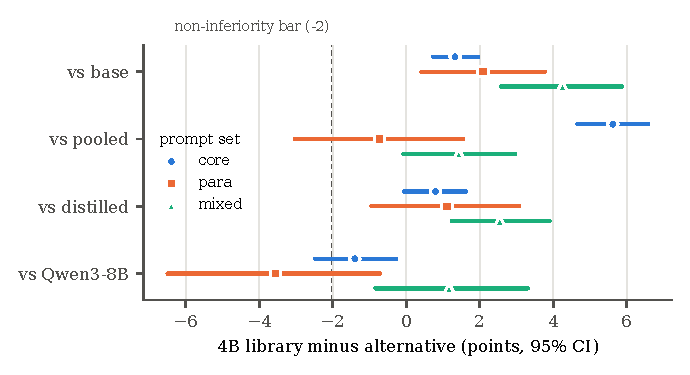
\includegraphics[width=0.62\linewidth]{figures/f2_library_vs_alternatives.pdf}
\caption{4B library minus each alternative, Part B test split, with 95\% paired-bootstrap intervals. The dashed line
is the non-inferiority bar. On core prompts the library is ahead of base and pooled; against distilled its
interval just includes 0, and it is behind Qwen3-8B. It is also behind 8B on reworded prompts.}
\label{fig:f2}
\end{figure}

\subsection{The next size up}
\label{sec:size}
The memory claim we set out to test was that a 4B library matches Qwen3-8B at about half the serving memory. It does
not, by our own bar (Figure~\ref{fig:f2}). The library-minus-8B difference is $-1.40$ \ci{-2.48}{-0.27} on core
prompts, $-3.56$ \ci{-6.49}{-0.71} and $-2.58$ \ci{-4.51}{-0.56} on the two reworded sets, and $+1.17$
\ci{-0.83}{3.31} on the multilingual set. H2 is inconclusive. At 4 bits the Part B test fails: AWQ 4B library minus
AWQ 8B is $-5.34$ \ci{-8.41}{-2.42} on reworded prompts (combined with Part C's fresh set, inconclusive; see
Table~\ref{tab:verdicts}). A later locked follow-up (Part D-A) paired an FP8 4B library
(7.13\,GB) with AWQ 8B (7.31\,GB): it is non-inferior on core ($+0.02$ \ci{-1.05}{1.13}; with a 2-point margin this
is not equivalence), passes on the multilingual set ($+2.53$ \ci{0.53}{4.69}), and is inconclusive on both reworded
sets ($-2.51$ \ci{-5.25}{0.48} and $-1.57$ \ci{-3.45}{0.33}). At matched memory a small library is close to a larger
model on standard phrasing and behind it, inconclusively or worse, on reworded phrasing.

\subsection{Fresh SQL and tool calling}
\label{sec:fresh}

\begin{table}[t]
\centering
\small
\begin{tabular}{lrr}
\toprule
System & Spider SQL (2,000) & BFCL live tools (1,292) \\
\midrule
Qwen3-4B (untouched) & 63.5 & 74.6 \\
Qwen3-8B (untouched) & 67.5 & 76.8 \\
Qwen3-8B AWQ & 66.8 & 76.1 \\
4B library (bf16) & 74.1 & 78.9 \\
4B library (FP8 base) & 73.6 & 78.6 \\
4B distilled & 74.5 & 79.2 \\
4B pooled & 75.1 & 79.4 \\
1.7B replay specialist & 69.0 & -- \\
\bottomrule
\end{tabular}
\caption{Part D-B, fresh test sets (execution accuracy for SQL, BFCL scoring for tools). Spider items whose
questions appear in our training data were removed before the lock (1,055 candidates dropped). Source:
\texttt{partd\_b\_embed-lr.json}.}
\label{tab:fresh}
\end{table}

Part D-B asked whether the SQL and tool gains survive on test sets built after the main study (Table~\ref{tab:fresh}),
using Spider \citep{yu2018spider} and BFCL live items.
The router sent every item to the right adapter. The 4B library beats the untouched 8B on Spider by 6.65 points
\ci{4.75}{8.52} ($n=2{,}000$) and the AWQ 8B by 7.30 \ci{5.43}{9.17}, and it passes the locked non-inferiority test
against 8B on BFCL live tool calls ($+2.09$ \ci{0.18}{3.97}; the interval also excludes 0). Two caveats limit what this shows. First, Spider's training split is in our SQL
training data, so these are in-distribution questions over unseen databases, not a new task. Second, a single 4B
model gets the same SQL gain: pooled 75.1 and distilled 74.5 against the library's 74.1. Third, we ran no
constrained or execution-guided SQL baseline. On a fresh set inside one
domain, the library's advantage is not a bigger gain; it is that the base is untouched for everything else
(Section~\ref{sec:libvs}).

\subsection{Nulls: replay, self-distillation and adapter rank}
\label{sec:nulls}
Three locked follow-ups found nothing to recommend. Training the adapters on self-distilled replay data (the base's
own answers to other domains' prompts) makes them far safer when applied to every request (always-on SQL adapter
$+4.11$ \ci{3.20}{5.02}, tools $+5.05$ \ci{4.19}{5.91} on core), but in a routed library it is slightly worse
($-0.50$ \ci{-0.82}{-0.21}, a fail) and costs SQL accuracy ($-2.52$ \ci{-4.30}{-1.04} on BIRD). Routing already hides
the damage that replay repairs. Adapter ranks 64 and 128 do not beat rank 16: every own-domain and composite test is
inconclusive (SQL $+1.17$ \ci{-0.26}{2.61} and $+1.48$ \ci{-0.17}{3.04}; composites $+0.18$ and $+0.14$). And plain
20\% replay added nothing measurable to LoRA adapters at 4B on the fresh reworded set ($-0.03$ \ci{-0.69}{0.62}).

\subsection{Niche tasks: METAR, MedCalc and a knowledge control}
\label{sec:niche}

\begin{table}[t]
\centering
\small
\begin{tabular}{lrrrrr}
\toprule
& \multicolumn{2}{c}{METAR (1,000)} & \multicolumn{2}{c}{MedCalc (1,100)} & Pre-Flight (240) \\
System & acc. & tokens & acc. & tokens & acc. \\
\midrule
4B zero-shot & 0.4 & 162 & 25.8 & 421 & 67.1 \\
4B few-shot & 36.2 & 144 & 65.2 & 361 & -- \\
4B few-shot + thinking & 61.3 & 1,175 & 77.3 & 2,186 & -- \\
8B zero-shot & 2.1 & 162 & 39.0 & 505 & 71.7 \\
8B few-shot & 41.7 & 144 & 65.7 & 448 & -- \\
8B thinking & 80.5 & 1,486 & 49.1 & 3,768 & 71.4 \\
8B few-shot + thinking & 83.2 & 1,664 & 79.8 & 2,209 & -- \\
14B zero-shot & 34.5 & 163 & 43.3 & 483 & 68.3 \\
32B zero-shot & 38.5 & 162 & 54.6 & 502 & 67.1 \\
32B thinking & 88.9 & 937 & 60.0 & 2,137 & 70.8 \\
\midrule
1.7B + task adapter & 99.1 & 143 & 45.8 & 511 & -- \\
4B + task adapter & 99.8 & 143 & 58.7 & 508 & -- \\
\bottomrule
\end{tabular}
\caption{Part D-C and D-F test results: accuracy (\%) and mean output tokens per item. METAR is scored as all 14
fields exact. Thinking and adapter rows are means over three seeds, except 32B thinking (one seed). Few-shot means
5 worked METAR examples, or the official one-shot MedCalc example for the item's calculator. Pre-Flight has no
training split, so it has no adapter or few-shot row; Pre-Flight with each task adapter is discussed in the text.
Sources: \texttt{partd\_c.json}, \texttt{partd\_f.json}.}
\label{tab:niche}
\end{table}

\begin{figure}[t]
\centering
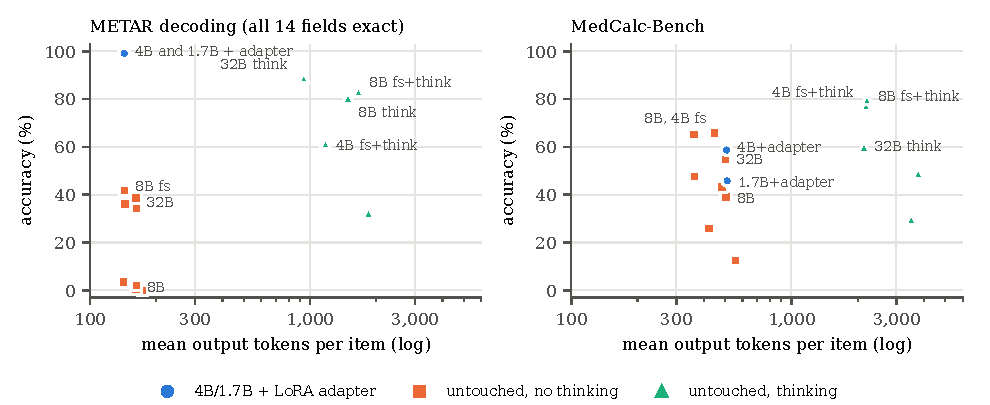
\includegraphics[width=\linewidth]{figures/f1_accuracy_vs_tokens.pdf}
\caption{Accuracy against mean output tokens per item. On METAR the adapter sits alone in the top-left corner: no
prompted untouched model reaches it at any token budget we tried. On MedCalc, few-shot prompting reaches it at a
similar budget, and few-shot prompting with thinking passes it at about four times the tokens.}
\label{fig:f1}
\end{figure}

Part D-C added three tasks Qwen is unlikely to have trained on heavily, all from public sources: METAR decoding
(raw aviation weather report to a 14-field JSON object; NWS/FAA reports from a public 2024 archive, train and test
stations disjoint, truth from a deterministic decoder cross-checked against an independent parser on 9,300 reports),
MedCalc-Bench v1.2 (patient note to a clinical calculation; 1,100 official test items, training notes shared with
test removed) and Pre-Flight, an aviation knowledge multiple-choice test with no training split, as a knowledge
control. Part D-F then gave the untouched models a fair chance: worked examples, thinking mode, and both.
Table~\ref{tab:niche} and Figure~\ref{fig:f1} show the results.

\paragraph{METAR favours training.} The 4B adapter gets all 14 fields right on 99.8\% of reports. The best untouched
8B condition, five worked examples plus thinking, reaches 83.2\%: the adapter is ahead by 16.67 points
\ci{15.00}{18.47}. Qwen3-32B with thinking reaches 88.9\% (adapter ahead by 10.93 \ci{9.07}{13.00}). Even the 1.7B
adapter beats the best 8B by 15.93 \ci{14.23}{17.73}. The adapter writes 143 output tokens per report; 8B with
examples and thinking writes 1,664 (11.6 times as many) and 32B with thinking writes 937. The untouched models'
errors are not only format: the zero-shot 8B writes times as ``0355'' instead of ``03:55'', and accepting that
lifts it only from 2.1\% to 18.5\%; the remaining misses are flight category, temperature and dewpoint, and wind
direction. The thinking rows are sampled (temperature 0.6, three seeds; one 8B thinking seed was paused and resumed
mid-run, Appendix~\ref{app:deviations}). That comparison is against thinking traces. Against constrained decoding, the cheaper alternative, the
adapter still leads by 10.2 points \ci{8.4}{12.2} (Section~\ref{sec:gate}). METAR also has
an exact non-learned solution: our labels come from a deterministic decoder that agrees with an independent parser on
9,300 reports, and in practice one would call such a decoder. We use METAR as a controlled probe of whether a small
model can learn a strict procedure, not as a recommendation to decode weather reports with a language model.

\paragraph{MedCalc reverses.} The 4B MedCalc adapter beats the untouched 4B by 32.85 points \ci{29.55}{36.00} and the
zero-shot 8B by 19.67 \ci{16.24}{22.91}, and beats the 8B with thinking ($+9.61$ \ci{6.70}{12.36}). But one worked
example closes the gap without training. The untouched 4B with the official one-shot example scores 65.2\%, above
its own adapter's 58.7\%; the 8B with few-shot examples beats the adapter by 7.06 \ci{4.03}{10.09}, and with few-shot
plus thinking by 21.18 \ci{18.58}{23.88}. Against 32B with thinking the adapter is level ($-1.33$ \ci{-4.70}{2.00}).
Dropping the five test items whose note contains an exemplar note changes no verdict (few-shot plus thinking
still ahead by 21.04 \ci{18.29}{23.71}). MedCalc items name the calculator, so one example of that calculator is
often all a model needs \citep{min2022demonstrations}; METAR has no such shortcut, because the skill is a whole
decoding table.

\paragraph{The knowledge control.} On Pre-Flight (240 items, descriptive only), 8B is 4.58 points above 4B
\ci{-0.83}{10.42}, but 32B zero-shot (67.1) is no better than 4B, so size is not clearly better here. Thinking did not
move the score measurably at any size (32B, one seed: $+3.75$ \ci{-1.67}{9.17}). Task adapters lowered the score when
applied to these questions: the 4B MedCalc adapter by 8.06 \ci{-12.50}{-2.92}, the 1.7B METAR adapter by 12.92
\ci{-17.08}{-8.89}. A skill adapter did not add knowledge, and applied outside its lane it removed some.

\subsection{Constrained-decoding gate (locked)}
\label{sec:gate}
The METAR comparison above is open to one objection: a practitioner who needs strict JSON would not prompt for it and
hope; they would constrain decoding to a schema \citep{willard2023outlines,dong2025xgrammar}. A schema fixes the
format by construction and needs no thinking trace, so it could narrow both the accuracy gap and the token gap. We
wrote and hashed this test before any of its outputs existed, after the Part D-C and D-F results were known.

\emph{Design.} Untouched Qwen3-8B and Qwen3-32B, served as before (vLLM, batch-invariant, bf16) with the XGrammar
backend constraining output to a JSON schema that encodes only what the METAR prompt states: the 14 keys, all
required, no extra keys, each field's type, the time as HH:MM, wind direction as an integer, ``VRB'' or null, and
cloud cover and flight category as their stated enumerations. All 1,300 dev and test gold references validate against
the schema, and the compiled grammar accepts every one of them. Schema arms get the same prompts with the instruction
to answer in a fenced block replaced by ``raw JSON, no code fence'', since the grammar cannot emit backticks. Six
primary schema arms: 8B and 32B, each zero-shot and five-shot (greedy, thinking off), plus 8B five-shot with
thinking and 32B zero-shot with thinking (sampled, seed 0, schema applied after the reasoning ends). Four
unconstrained controls (8B and 32B, zero-shot and five-shot) run on the same server. Every arm is scored on the same
1,000 test reports by the same scorer. \emph{Stop rules.} The unconstrained zero-shot 8B must reproduce the stored
Part D-C outputs byte for byte. Every non-truncated output of a schema arm must parse, validate and carry no fence;
otherwise the grammar was not applied and the result is void. A 30-item dev smoke test can change one setting
(whitespace in the grammar, if any schema arm truncates more than 2 of 30 items).

\emph{Tests.} G1: the 4B adapter beats the best 8B schema arm. G2: it beats the best 32B schema arm. G3, which
decides the headline, applies two one-sided tests with a 2.0-point margin to $d$ = adapter minus the best of the six
schema arms: the schema arm is ``ahead'' if the interval for $d$ lies below 0 and ``equivalent'' if it lies inside
$(-2.0, 2.0)$. Choosing the best arm after the fact makes G1 and G2 harder for the adapter and makes equivalence
easier. G4 reports each schema arm minus its unconstrained control. A station-cluster bootstrap repeats G1 to G3 as a
sensitivity check. \emph{Decision rule}, fixed in advance: void if the parity or output checks fail or an arm is
missing; if the schema arm is ahead or equivalent, the METAR training result is withdrawn and METAR joins MedCalc as a
task where training was not needed; if G1 and G2 pass and the lower end of the interval for $d$ is above 2.0, we
report only that format-only constrained decoding did not come within 2 points of the adapter; anything else is
reported as $d$ with its interval and no direction word. \emph{Prediction} (written before any output): the schema
fixes format only, the best schema arm is 32B with thinking at 86 to 91, G1 and G2 pass, and the non-thinking schema
arms use about as many tokens as the adapter.

\emph{What the gate cannot show.} The schema encodes only what the prompt states. Most remaining errors of the
prompted models are already inside valid JSON (wrong flight category, temperature or ceiling), so a format constraint
is not expected to fix them, and a pass would mean that formatting is not the explanation, not that no non-training
method could match the adapter. A schema that encodes the flight-category rule, a 4B-plus-schema arm and the
deterministic decoder itself are not in the gate (the decoder produced the labels, so it scores 100 by construction).

\emph{Result.} The run used 2.51 GPU-hours on one RTX PRO 6000. Parity held (1,000 of 1,000 outputs identical to
the stored zero-shot 8B run), and every non-truncated schema-arm output parsed, validated and carried no fence (one
truncation in 1,000 for 32B with thinking). Three deviations were logged, none of which changed an arm, prompt, schema or
test (Appendix~\ref{app:deviations}). Table~\ref{tab:gate} gives the scores.

\begin{table}[t]
\centering
\small
\begin{tabular}{lrrr}
\toprule
System (METAR test, $n=1{,}000$) & All fields (\%) & No schema & Tokens/item \\
\midrule
4B + METAR adapter (3 training seeds) & 99.8 & -- & 143 \\
8B zero-shot + schema & 20.4 & 2.1 & 159 \\
8B five-shot + schema & 42.9 & 41.7 & 140 \\
8B five-shot + thinking + schema (seed 0) & 84.2 & 82.9$^\dagger$ & 1,639 \\
32B zero-shot + schema & 38.1 & 38.6 & 158 \\
32B five-shot + schema & 66.2 & 67.6 & 139 \\
32B thinking + schema (seed 0) & 89.6 & 88.9$^\dagger$ & 935 \\
\bottomrule
\end{tabular}
\caption{Constrained-decoding gate. Schema arms use XGrammar with schema v1. ``All fields'': all 14 fields exact.
``No schema'': the same system on the same server without the schema. $^\dagger$Part F runs on another Station
without a reasoning parser.}
\label{tab:gate}
\end{table}

G1: the adapter beats the best 8B schema arm (five-shot with thinking) by 15.63 \ci{13.33}{17.90}, PASS. G2: it beats
the best 32B schema arm (thinking) by 10.23 \ci{8.40}{12.23}, PASS. G3: $d$ = 10.23 \ci{8.40}{12.23}, not
equivalent. A station-cluster bootstrap gives \ci{7.51}{13.01} for $d$ and the same verdicts. Under the frozen rule
the METAR result stands, and we state it only in the allowed form: with this schema under XGrammar, no untouched 8B
or 32B arm came within 2 points of the adapter. The schema itself helped only where the error was format: zero-shot
8B gains 18.30 \ci{15.90}{20.70}, almost all from the time format, while the other same-server differences lie
between $-1.40$ and $+1.20$ points. Tokens: constrained arms without thinking write about as many tokens as the
adapter (0.97 to 1.11 times) and trail it by 33 to 79 points; the best constrained arm writes 935 tokens, 6.5 times
the adapter's. Because every constrained arm is more than 2 points behind, the token comparison that matters remains
the one against thinking, and we label it that way. Every arm landed in its predicted range.

\section{Discussion}

A practical rule is consistent with these results, though none of them establishes it. If one worked example can
show the procedure, as with a named MedCalc calculator, try the example first: it matched or beat training here. If
the procedure is too large for an example, as with METAR's decoding table, a small adapter beat every prompted
untouched model we tried, with or without constrained decoding. On a fresh SQL set any 4B fine-tune (library,
pooled or distilled) beat the untouched 8B, so that result supports fine-tuning, not routing in particular. Adapters
did not supply knowledge.

The always-on base matters more than the adapters. Every arrangement that replaced the base everywhere (pooled
fine-tuning, merged specialists, a specialist used for every request) lost skills the base already had. In an
exploratory read of the 1.7B dev results, the code adapter applied to every request dropped math from 77.3 to 52.8
and the composite from 55.3 to 48.2, while the same adapter behind the router left math untouched. Routing is what
makes adapters safe, and a cheap router is enough when the domains are distinct.

A distilled single model is the strongest competitor we tested. It got the library's SQL gain on Spider and tied the
library on most sets. When the domain list is fixed, distilling may be the simpler deployment; the library's case
rests on adding or removing a skill without retraining anything else.

\section{Limitations}
\begin{itemize}
\item One model family. Every model is Qwen3. A second family is the most important missing replication.
\item Template overlap. SQL, tools, math and translation training data share the core prompt templates; the
  paraphrase sets are the clean test, and they are where the library's results are weakest. MedCalc test items share
  calculator families with training, and METAR training and test share the report format (with disjoint stations).
\item Named calculators. MedCalc prompts name the calculator. A deployment that must first pick the
  calculator from a raw note was not tested.
\item Locked follow-ups, local timestamps. Part D was designed after earlier results were known. All
  manifests and timestamps are local records: \emph{Preregistered locally; timestamps not externally verifiable.}
\item One schema, one backend. The METAR constrained-decoding gate tests one prompt-faithful, format-only schema
  with one backend (XGrammar) and one sampling seed for the thinking arms. A schema or decoder that encodes METAR's
  rules was not tested.
\item Scale. We test 1.7B and 4B libraries against 8B, with 14B and 32B only on the niche tasks. We make no
  claim about larger bases.
\item Interval width. The bootstrap resamples items around three-seed means, so intervals omit training-seed
  variance, and Spider items are not clustered by database. Some intervals are therefore narrower than a
  seed-and-cluster bootstrap would give.
\item Same-family paraphraser and pretraining contamination. The reworded sets were written by a Qwen-family model.
  We removed Spider items that overlap our fine-tuning data but did not measure overlap with Qwen's pretraining data;
  METAR and Spider are both old public formats.
\item Deviations. Every logged deviation from the locked files is summarized in Appendix~\ref{app:deviations}.
\item Composite weighting and power. Composites weight domains equally; reworded sets have 590 and 1,562
  items, and several inconclusive verdicts reflect their width.
\end{itemize}

\section*{AI assistance disclosure}
AI agents designed, ran, and drafted this work under PI supervision. The PI verified every number and is responsible
for every claim.

\section*{Data and code availability}
Code, configurations, frozen manifests, per-item scores and the public-source niche-task builders are prepared for
release; the release is pending the author's approval. MedCalc-Bench-derived data is CC BY-SA 4.0 and Pre-Flight is
MIT (Airside Labs); METAR reports are US government observations. No proprietary or patient data was used.

\bibliographystyle{plainnat}
\bibliography{refs}

\appendix

\section{Determinism and evaluation hygiene}
\label{app:determinism}
\paragraph{Batched greedy decoding is not repeatable.} Rerunning the same greedy evaluation of Qwen3-1.7B on the same
GPU and server gave identical outputs for 1,927 of 6,016 MMLU-Pro items (32\%) and 67 of 250 MATH-500 items (27\%);
MATH-500 moved from 71.6 to 73.2. Batch composition changes floating-point reductions, and one changed token
changes the rest of the answer. This noise is the same size as many published model differences.
\paragraph{Batch-invariant kernels fix it.} With vLLM's batch-invariant mode, two greedy runs were identical on 1,179
of 1,179 prompts, and outputs were identical across two DGX Spark (GB10) systems and a GB300 on the same 1,179
prompts. Before the Part B test pass, the two RTX PRO 6000 evaluators produced byte-identical outputs on all 9,262
dev items of the base model. Any of our GPUs could therefore score any arm.
\paragraph{Token caps truncate silently.} With 512--1,024-token caps, greedy decoding truncated 21--29\% of MATH-500
and MMLU-Pro answers; raising the cap to 4,096 moved Qwen3-1.7B MMLU-Pro from 37.9 to 43.8.
\paragraph{A scorer bug.} The IFEval checkers draw missing arguments from Python's global random state, so a score
depended on how many items had been scored before it (69.63 against 69.26 on identical outputs). We seed per item.

\section{Deviations from the locked files}
\label{app:deviations}
Part B and Part C recorded no deviations. The Part D log (\texttt{content/PART\_D\_DEVIATIONS.md}) has seven entries.
(1) Two BFCL live prompts longer than 4,096 tokens returned errors for every model and were removed by length only
(1,294 to 1,292 items) before any score was used. (2, 4) Clock notes: three locked files state write times that were
off by up to about an hour; the notebook's \texttt{date} stamps are authoritative, and every file was still locked before
outputs on its data existed. (3) An operational jobs file gained jobs after the lock; its locked copy is hashed. (5)
An evaluation queue believed stopped kept running through a pause; jobs hit by a host reboot were rerun in full, and
under batch-invariant greedy decoding a rerun gives the same outputs. (6) Seed-mean Part D-C scores were seen before
the analysis script was written; the script's tests are exactly those of the locked addendum, and it was hashed
before its first run. (7) The Part D-F queue was paused and resumed with the same frozen files; one sampled 8B
thinking seed was mid-run, so its later items were drawn after the resume.

The constrained-decoding gate log (\texttt{content/PART\_G\_DEVIATIONS.md}) has three entries, all written before any
schema arm produced test output. (1) Serving path: requests went through a separate research-only LiteLLM router with
the same image and only the gate's routes, instead of the production router named in the locked card, and the GPU was
selected by verified device UUID instead of by index. No arm, prompt, schema, decoding setting, scorer, test or
decision rule changed.
(2) Smoke-check bug and a fired stop rule, after the development smoke and before any test-split output. The
smoke-check script read the run name from the wrong path component, so it treated every run as unconstrained, printed
PASS without applying any schema rule, and the launcher wrote its smoke-ok marker on that false pass. The script was
fixed (with a regression test) and the frozen smoke rules were then applied to the stored smoke outputs. On those
outputs no schema arm had a truncated, unparseable, schema-invalid or fenced output (0 of 180 items across the six
schema arms). The frozen null-branch rule did fire. That rule said: if a schema arm writes a number where the gold
value is null, stop, investigate, and make no automatic change. It fired for the two zero-shot schema arms only
(8B and 32B): \texttt{wind\_dir\_deg} is null for 5 of the 30 gold smoke items (calm wind, 00000KT) and both arms wrote
0 for all five. The investigation used stored outputs only (no new generation). The unconstrained zero-shot 8B and
32B runs also write 0 on all 268 calm test reports (0 of 268 null), while unconstrained 8B five-shot writes null on
268 of 268. Under the same grammar, the four other schema arms write null on the smoke items (five-shot 5 of 5;
thinking 4 of 5 and 5 of 5), and XGrammar 0.2.7 accepts every gold null (1,300 of 1,300 checked). The grammar
therefore had not lost its null branch: writing 0 for calm wind is the zero-shot models' own reading of the prompt,
and it is a real error the gate should score. Decision: because the rule's purpose was to detect a lost null branch
and that purpose was shown not to apply, the main run proceeded with every arm unchanged; the smoke-ok marker was
rewritten by hand to cite this log entry, and the smoke outputs were kept as development-only records with no scores
computed. The PI accepted this deviation on 2026-11-14. The calm-wind error is scored in the results above, not
repaired, excluded or rescored.
(3) The aggregation step failed on an import path (\texttt{python -P} drops the working directory from
\texttt{sys.path}) after the parity run had generated all 1,000 of its outputs and before any schema arm had started.
The call was fixed by passing \texttt{PYTHONPATH} explicitly; the parity run was aggregated with the same command
and checked with the launcher's own parity test (1,000 of 1,000 outputs identical to the stored run, score 2.1 in
both), and the queue relaunched without regenerating those outputs.

\section{Development-split findings (Part A, exploratory)}
\label{app:parta}
All Part A numbers are on the dev split and informed the Part B design. Merging the six 1.7B specialists (averaging
or TIES) scored 48.8--51.5 against 53.1--53.5 for pooled, and lost the SQL gain. Specialists trained from the Base
(non-instruct) checkpoint beat pooled training when routed, but broke on reworded prompts (the Base-init code
specialist fell from 71.7 to 33.3 on reworded MBPP items); 20\% replay restored it to about 60. LoRA adapters trained
from a Base checkpoint never learned to emit the end-of-turn token and were dropped. Domain-tagging the pooled model
recovered none of the library's advantage ($+0.4$, within seed noise).

\end{document}
